\documentclass[11pt,a4paper]{article}
\usepackage[utf8]{inputenc}
\usepackage[spanish]{babel}
\usepackage{geometry}
\geometry{top=3cm, bottom=3cm, left=2.5cm, right=2.5cm}
\usepackage{graphicx}
\usepackage{booktabs}
\usepackage{listings}
\usepackage{xcolor}
\usepackage{hyperref}
\usepackage{titlesec}
\usepackage{enumitem}
\usepackage{fancyhdr}

\definecolor{codegreen}{rgb}{0,0.6,0}
\definecolor{codegray}{rgb}{0.5,0.5,0.5}
\definecolor{codepurple}{rgb}{0.58,0,0.82}
\definecolor{backcolour}{rgb}{0.95,0.95,0.92}

\lstdefinestyle{mystyle}{
    backgroundcolor=\color{backcolour},   
    commentstyle=\color{codegreen},
    keywordstyle=\color{magenta},
    numberstyle=\tiny\color{codegray},
    stringstyle=\color{codepurple},
    basicstyle=\ttfamily\footnotesize,
    breakatwhitespace=false,         
    breaklines=true,                 
    captionpos=b,                    
    keepspaces=true,                 
    numbers=left,                    
    numbersep=5pt,                  
    showspaces=false,                
    showstringspaces=false,
    showtabs=false,                  
    tabsize=2
}
\lstset{style=mystyle}

\pagestyle{fancy}
\fancyhf{}
\rhead{Sistema de Gestión de Emergencias Universitarias}
\lfoot{Monorepo Hackatón}
\rfoot{Página \thepage}

\title{
  \textbf{Sistema de Gestión de Emergencias Universitarias}\\
  \large Informe de Desarrollo e Integración (Pisos 1-3)
}
\author{
  \textbf{Backend:} Joaquín Felipez Rojas \& David Willy Cruz \\
  \textbf{Frontend:} Nicolás Reguerin\& Jhoan Calderon
}
\date{18 de Junio de 2026}

\begin{document}

\maketitle
\tableofcontents
\newpage

\section{Información General}
\begin{itemize}
    \item \textbf{Nombre del Proyecto:} Sistema de Gestión de Emergencias Universitarias
    \item \textbf{Integrantes del Equipo:}
    \begin{itemize}
        \item \textbf{Desarrollo Backend:} Joaquín Felipez Rojas y David Willy Cruz.
        \item \textbf{Desarrollo Frontend:} Nicolás y Jhoan.
    \end{itemize}
    \item \textbf{Sprint o Fase Desarrollada:} Pisos 1 (Cimentación), 2 (Estructura - Autenticación) y 3 (Core - Gestión de Incidentes).
\end{itemize}

\section{Funcionalidad Implementada}
\subsection{Descripción de la Funcionalidad}
El sistema permite que los miembros de la comunidad universitaria reporten de manera ágil situaciones de emergencia dentro del campus (como incendios, cortes de energía, accidentes, inundaciones, problemas de seguridad u otros). Una vez reportados, estos incidentes quedan registrados con su tipo, ubicación exacta, severidad y descripción para permitir un seguimiento riguroso.

\subsection{Objetivo}
Proveer una plataforma centralizada y eficiente para el registro, asignación, seguimiento y auditoría de incidentes y emergencias universitarias, logrando coordinar una atención oportuna y registrar un historial fiable para futuras auditorías.

\subsection{Requerimientos Involucrados}
\begin{itemize}
    \item \textbf{RF-001 (Reportar Incidente):} El usuario debe poder reportar un incidente especificando tipo, severidad, ubicación y descripción.
    \item \textbf{RF-002 (Ver Detalle de Incidente):} El usuario debe poder ver la información completa de un incidente.
    \item \textbf{RF-003 (Listar Incidentes):} El administrador debe poder listar todos los incidentes con paginación.
    \item \textbf{RF-008 (Autenticación):} Los usuarios deben poder iniciar sesión en el sistema.
    \item \textbf{RF-009 (Historial de Cambios):} El sistema debe registrar cada cambio de estado y responsable del incidente.
    \item \textbf{RNF-004 y RNF-005 (Seguridad):} Restricción de acceso solo a usuarios autenticados y validación de roles en endpoints críticos.
    \item \textbf{RN-003:} El tipo de incidente debe ser: \textit{incendio, corte\_energía, accidente, inundación, seguridad, otro}.
    \item \textbf{RN-004:} La severidad debe ser: \textit{baja, media, alta, crítica}.
\end{itemize}

\section{Desarrollo Realizado}
\subsection{Arquitectura Utilizada}
La solución utiliza una arquitectura de Monorepo estructurada de la siguiente manera:
\begin{itemize}
    \item \textbf{Backend (API RESTful):} NestJS escrito en TypeScript, modular, con inyección de dependencias. Usa \textbf{Prisma ORM} para conectarse de forma segura y tipada a una base de datos relacional.
    \item \textbf{Base de Datos:} \textbf{PostgreSQL} que reside en un contenedor Docker, garantizando un entorno reproducible y limpio.
    \item \textbf{Frontend (Interfaz de Usuario):} React + Vite para compilación instantánea y desarrollo ágil. Para los estilos y UI se utiliza Tailwind CSS v4, Base UI / Radix UI y componentes shadcn/ui v2. La gestión de estado asíncrono se realiza mediante TanStack Query y los formularios se manejan con React Hook Form + Zod.
\end{itemize}

\subsection{Clases o Módulos Desarrollados}
El sistema cuenta con las siguientes clases y entidades principales:
\begin{enumerate}
    \item \textbf{Usuario (User):} Modelo base para almacenar credenciales (email, hash de contraseña bcrypt), estado y datos generales.
    \item \textbf{Rol (Role):} Modelo para gestionar dinámicamente los roles (\textit{admin, responder, user}).
    \item \textbf{Incidente (Incident):} Entidad que almacena los detalles específicos del reporte (título, descripción, tipo, severidad, estado, ubicación).
    \item \textbf{Auditoría (AuditLog):} Entidad encargada de registrar cronológicamente todas las acciones y cambios de estado efectuados sobre los incidentes.
    \item \textbf{Área Campus (CampusArea):} Lugares específicos del campus que facilitan la localización geográfica del incidente.
\end{enumerate}
\subsection{Capturas del Sistema Funcionando}
\begin{figure}[h!]
    \centering
    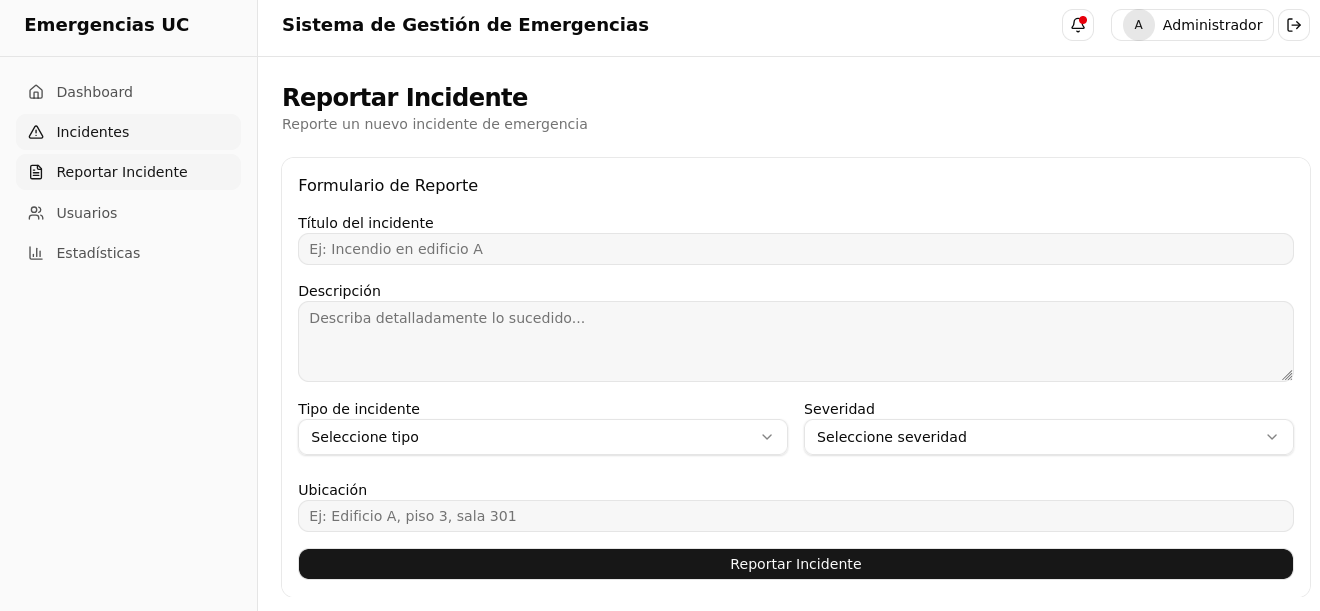
\includegraphics[width=0.9\textwidth]{captura-formulario.png}
    \caption{Formulario de Registro y Reporte de Incidentes en React + Tailwind v4.}
\end{figure}

\newpage

\section{Actividades de Debugging}
Durante el desarrollo e integración de las ramas en la rama central \texttt{dev}, se identificaron y resolvieron los siguientes problemas críticos:

\subsection{Error 1: Clases border-border, bg-background, text-foreground no existen}
\begin{itemize}
    \item \textbf{Descripción:} Fallo en la compilación de PostCSS en Vite indicando que las clases de diseño de shadcn no se encontraban.
    \item \textbf{Causa:} El setup de shadcn se inicializó asumiendo Tailwind CSS v4, pero la aplicación usaba Tailwind CSS v3.
    \item \textbf{Solución:} Se instaló Tailwind v4 y su plugin oficial para Vite (\texttt{@tailwindcss/vite}), se actualizó \texttt{index.css} y se eliminaron los archivos de configuración obsoletos v3 (\texttt{tailwind.config.js} y \texttt{postcss.config.js}).
\end{itemize}

\subsection{Error 2: Conflictos al fusionar p1-frontend-base con dev}
\begin{itemize}
    \item \textbf{Descripción:} Múltiples conflictos en \texttt{package.json}, \texttt{App.tsx} e \texttt{index.css}.
    \item \textbf{Causa:} Dos ramas de tareas paralelas del Piso 1 colisionaron al modificar el mismo árbol de directorios del frontend.
    \item \textbf{Solución:} Se resolvieron manualmente los archivos conservando la base tecnológica moderna (Tailwind v4 y Base UI), re-instalando las dependencias necesarias.
\end{itemize}

\subsection{Error 3: Módulos de backend no encontrados tras merge}
\begin{itemize}
    \item \textbf{Descripción:} Errores del tipo \textit{"Cannot find module '@nestjs/jwt'"}.
    \item \textbf{Causa:} Las dependencias requeridas para la autenticación se instalaron localmente pero no se commitearon ni registraron en el lockfile general.
    \item \textbf{Solución:} Se ejecutó \texttt{pnpm install} para reconstruir y sincronizar el archivo de bloqueo de pnpm de forma correcta.
\end{itemize}

\subsection{Error 4: Guards de ruta apuntando a la redirección anterior}
\begin{itemize}
    \item \textbf{Descripción:} Los guards redirigían al usuario no autenticado a \texttt{/login} en lugar de \texttt{/auth}.
    \item \textbf{Causa:} Al unificar las pantallas de autenticación en \texttt{/auth} con Tabs, las redirecciones estáticas de los guards no fueron actualizadas.
    \item \textbf{Solución:} Se modificó la dirección en \texttt{ProtectedRoute.tsx}, \texttt{AdminRoute.tsx} y \texttt{ResponsableRoute.tsx} para usar el endpoint correcto.
\end{itemize}

\section{Pruebas Realizadas}
Se validó la estabilidad del monorepo mediante pruebas locales exhaustivas:
\begin{itemize}
    \item \textbf{Build check del Monorepo:} Ejecución de \texttt{pnpm build} garantizando que tanto la aplicación frontend como backend transpilen a JavaScript nativo sin errores de empaquetado.
    \item \textbf{Verificación de Tipos estáticos:} Ejecución de \texttt{pnpm check-types} garantizando integridad estricta en todas las interfaces, esquemas Zod y controladores.
    \item \textbf{Flujo de Autenticación:} Pruebas de generación y firma de tokens JWT junto con la decodificación por parte del backend y almacenamiento en cliente mediante cookies/localStorage.
\end{itemize}

\newpage
\section{Conclusiones}
\begin{itemize}
    \item \textbf{Lecciones Aprendidas:} La importancia de tener un flujo de Git bien planificado y realizar sincronizaciones continuas con la rama \texttt{dev} para prevenir conflictos masivos en dependencias y configuración. Además, la adopción de Tailwind CSS v4 requiere actualizar la configuración clásica a la nueva sintaxis basada en CSS nativo.
    \item \textbf{Mejoras Futuras:} Implementación de comunicación bidireccional por WebSockets para notificaciones en tiempo real, e integración de geolocalización real mediante mapas interactivos.
\end{itemize}

\section{Anexos}
\subsection{Enlace del Repositorio}
El código fuente completo del proyecto y su historial de desarrollo se encuentra disponible en:
\begin{itemize}
    \item \textbf{Repositorio Principal (GitHub):} \url{https://github.com/Joaquinfr87/hackaton}
\end{itemize}

\subsection{Script de Base de Datos}
El siguiente script en SQL representa la base de datos PostgreSQL generada por las migraciones de Prisma para el monorepo:
\begin{lstlisting}[language=SQL]
-- CreateTable
CREATE TABLE "users" (
    "id" TEXT NOT NULL,
    "name" TEXT NOT NULL,
    "email" TEXT NOT NULL,
    "password_hash" TEXT NOT NULL,
    "phone" TEXT,
    "is_active" BOOLEAN NOT NULL DEFAULT true,
    "created_at" TIMESTAMP(3) NOT NULL DEFAULT CURRENT_TIMESTAMP,
    "updated_at" TIMESTAMP(3) NOT NULL,
    CONSTRAINT "users_pkey" PRIMARY KEY ("id")
);

-- CreateTable
CREATE TABLE "roles" (
    "id" TEXT NOT NULL,
    "name" TEXT NOT NULL,
    "description" TEXT,
    "created_at" TIMESTAMP(3) NOT NULL DEFAULT CURRENT_TIMESTAMP,
    CONSTRAINT "roles_pkey" PRIMARY KEY ("id")
);

-- CreateTable
CREATE TABLE "user_roles" (
    "user_id" TEXT NOT NULL,
    "role_id" TEXT NOT NULL,
    CONSTRAINT "user_roles_pkey" PRIMARY KEY ("user_id","role_id")
);

-- CreateTable
CREATE TABLE "campus_areas" (
    "id" TEXT NOT NULL,
    "name" TEXT NOT NULL,
    "description" TEXT,
    "location" TEXT,
    "created_at" TIMESTAMP(3) NOT NULL DEFAULT CURRENT_TIMESTAMP,
    CONSTRAINT "campus_areas_pkey" PRIMARY KEY ("id")
);

-- CreateTable
CREATE TABLE "incidents" (
    "id" TEXT NOT NULL,
    "title" TEXT NOT NULL,
    "description" TEXT NOT NULL,
    "type" TEXT NOT NULL,
    "severity" TEXT NOT NULL,
    "status" TEXT NOT NULL DEFAULT 'reported',
    "location" TEXT NOT NULL,
    "reported_by_id" TEXT NOT NULL,
    "assigned_to_id" TEXT,
    "area_id" TEXT,
    "created_at" TIMESTAMP(3) NOT NULL DEFAULT CURRENT_TIMESTAMP,
    "updated_at" TIMESTAMP(3) NOT NULL,
    CONSTRAINT "incidents_pkey" PRIMARY KEY ("id")
);

-- CreateTable
CREATE TABLE "audit_logs" (
    "id" TEXT NOT NULL,
    "incident_id" TEXT NOT NULL,
    "user_id" TEXT NOT NULL,
    "action" TEXT NOT NULL,
    "old_status" TEXT,
    "new_status" TEXT,
    "comment" TEXT,
    "created_at" TIMESTAMP(3) NOT NULL DEFAULT CURRENT_TIMESTAMP,
    CONSTRAINT "audit_logs_pkey" PRIMARY KEY ("id")
);

-- CreateIndex
CREATE UNIQUE INDEX "users_email_key" ON "users"("email");
CREATE UNIQUE INDEX "roles_name_key" ON "roles"("name");
CREATE UNIQUE INDEX "campus_areas_name_key" ON "campus_areas"("name");
\end{lstlisting}

\newpage
\subsection{Historial de Commits (Git Log)}
A continuación se detallan los últimos commits registrados en la rama de desarrollo:
\begin{lstlisting}[language=bash]
d96a685 Merge remote-tracking branch 'origin/feature/p3-reportar-incidente' into dev
7502b2d Merge remote-tracking branch 'origin/feature/p3-incidents-api' into dev
99d4ad2 Merge remote-tracking branch 'origin/p3-auditoria-servicio' into dev
44638a9 feat: creacion de CRUD de incidentes en NestJs
4bf432a feat(p3): crear formulario para reportar incidente con validacion de zod
084b75f p2(fix): Fix de rutas protegidas
b9be72a Feat: implementacion servicio de auditoria
fe4381b Merge pull request #9 from Joaquinfr87/feature/p2-auth-guard-frontend
3ca0943 feat(p2): implementar guards de rutas por rol y redireccion de autenticacion
6ab90bb feat(p2): implement roles service, guard, and decorator
393ce12 p2(fix): se unio la rama auth-pages con la rama auth-hook, se resolvio los conflictos
e49c20e Merge feature/p2-auth-pages into dev
634846a Merge pull request #8 from Joaquinfr87/feature/p2-auth-hook
458839c p2(feat): se anadio de hook personalizado useAuth con tanstack query
a13017c feat(p2): unificar login y register con tabs
\end{lstlisting}

\end{document}
